\section[Matrices de conexiones]{Matrices de conexiones modulares \sectionmark{Matrices de conexiones}}
\sectionmark{Matrices de conexiones}
\label{sec:patchbay}

Un sintetizador modular típico, comunica sus módulos por medio de cables que el usuario conecta (fig. \ref{fig:sintetizador_modular}). Los términos \textit{patch} y \textit{patcher} se usan habitualmente para designar un conjunto de conexiones entre módulos, no solo en el caso del audio analógico, sino también del mundo digital. Sintetizadores de propósito general como \textit{Pure Data} o \textit{MAX}, siguen este paradigma de <<patchear>> entradas y salidas con cables virtuales (fig. \ref{fig:puredata_modular}). Sin embargo, si hay algo que caracteriza a los sintetizadores de EMS, es la forma particular en la que se realizan las conexiones entre sus módulos. 
%	
%\begin{figure}
%	\centering
%	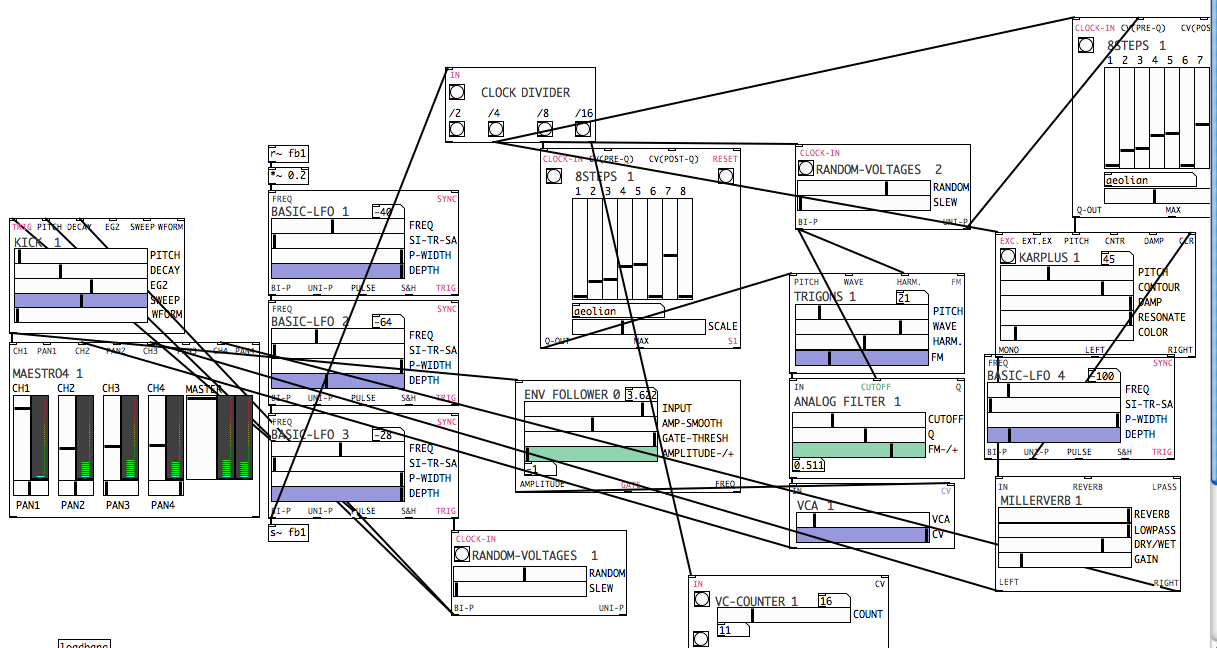
\includegraphics[width=0.7\textwidth]{images/pd_patch_example}
%	\caption[\textit{Patch de ejemplo diseñado en \textit{Pure Data}}]{\textit{Patch de ejemplo diseñado en \textit{Pure Data}}}
%	\label{fig:pd_patch_example}
%\end{figure}
%	

No es necesario el uso de un solo cable para ordenar las entradas y salidas. En lugar de tener un único conector para cada salida o entrada, Synthi 100 tiene dos matrices bidimensionales cuyas ordenadas representan a las salidas y las abcisas las entradas de todos los módulos. Cada uno de sus nodos representa, por tanto, una conexión posible, a modo de coordenada. Las matrices del Synthi 100 del GME de Cuenca tienen unas dimensiones de 66 columnas por 60 filas, si bien algunas de estas no tienen ninguna conexión en este momento. En la matriz de \textit{Audio Control} existen 59 filas y 64 columnas, haciendo un total de 3776 conexiones individuales posibles. La de \textit{Voltage Control}, asimismo, 56 filas por 65 columnas, con un total de 3640 individuales posibles.

La conexión se realiza por medio de unas clavijas que, al introducirse en la conexión hembra, cierran el circuito. La limpieza visual de las conexiones es indiscutible respecto al paradigma del sintetizador modular por cables, especialmente cuando el número de conexiones es significativa; es muy fácil de reflejar en tablas sobre papel (fig. \ref{fig:dope_sheet_GME}), incluso es posible escribirlo con coordenadas numéricas, ya que cada salida o entrada tiene un número único asignado (fig. \ref{fig:patchbay_audio_vista_gral}).

\begin{figure}
	\centering
	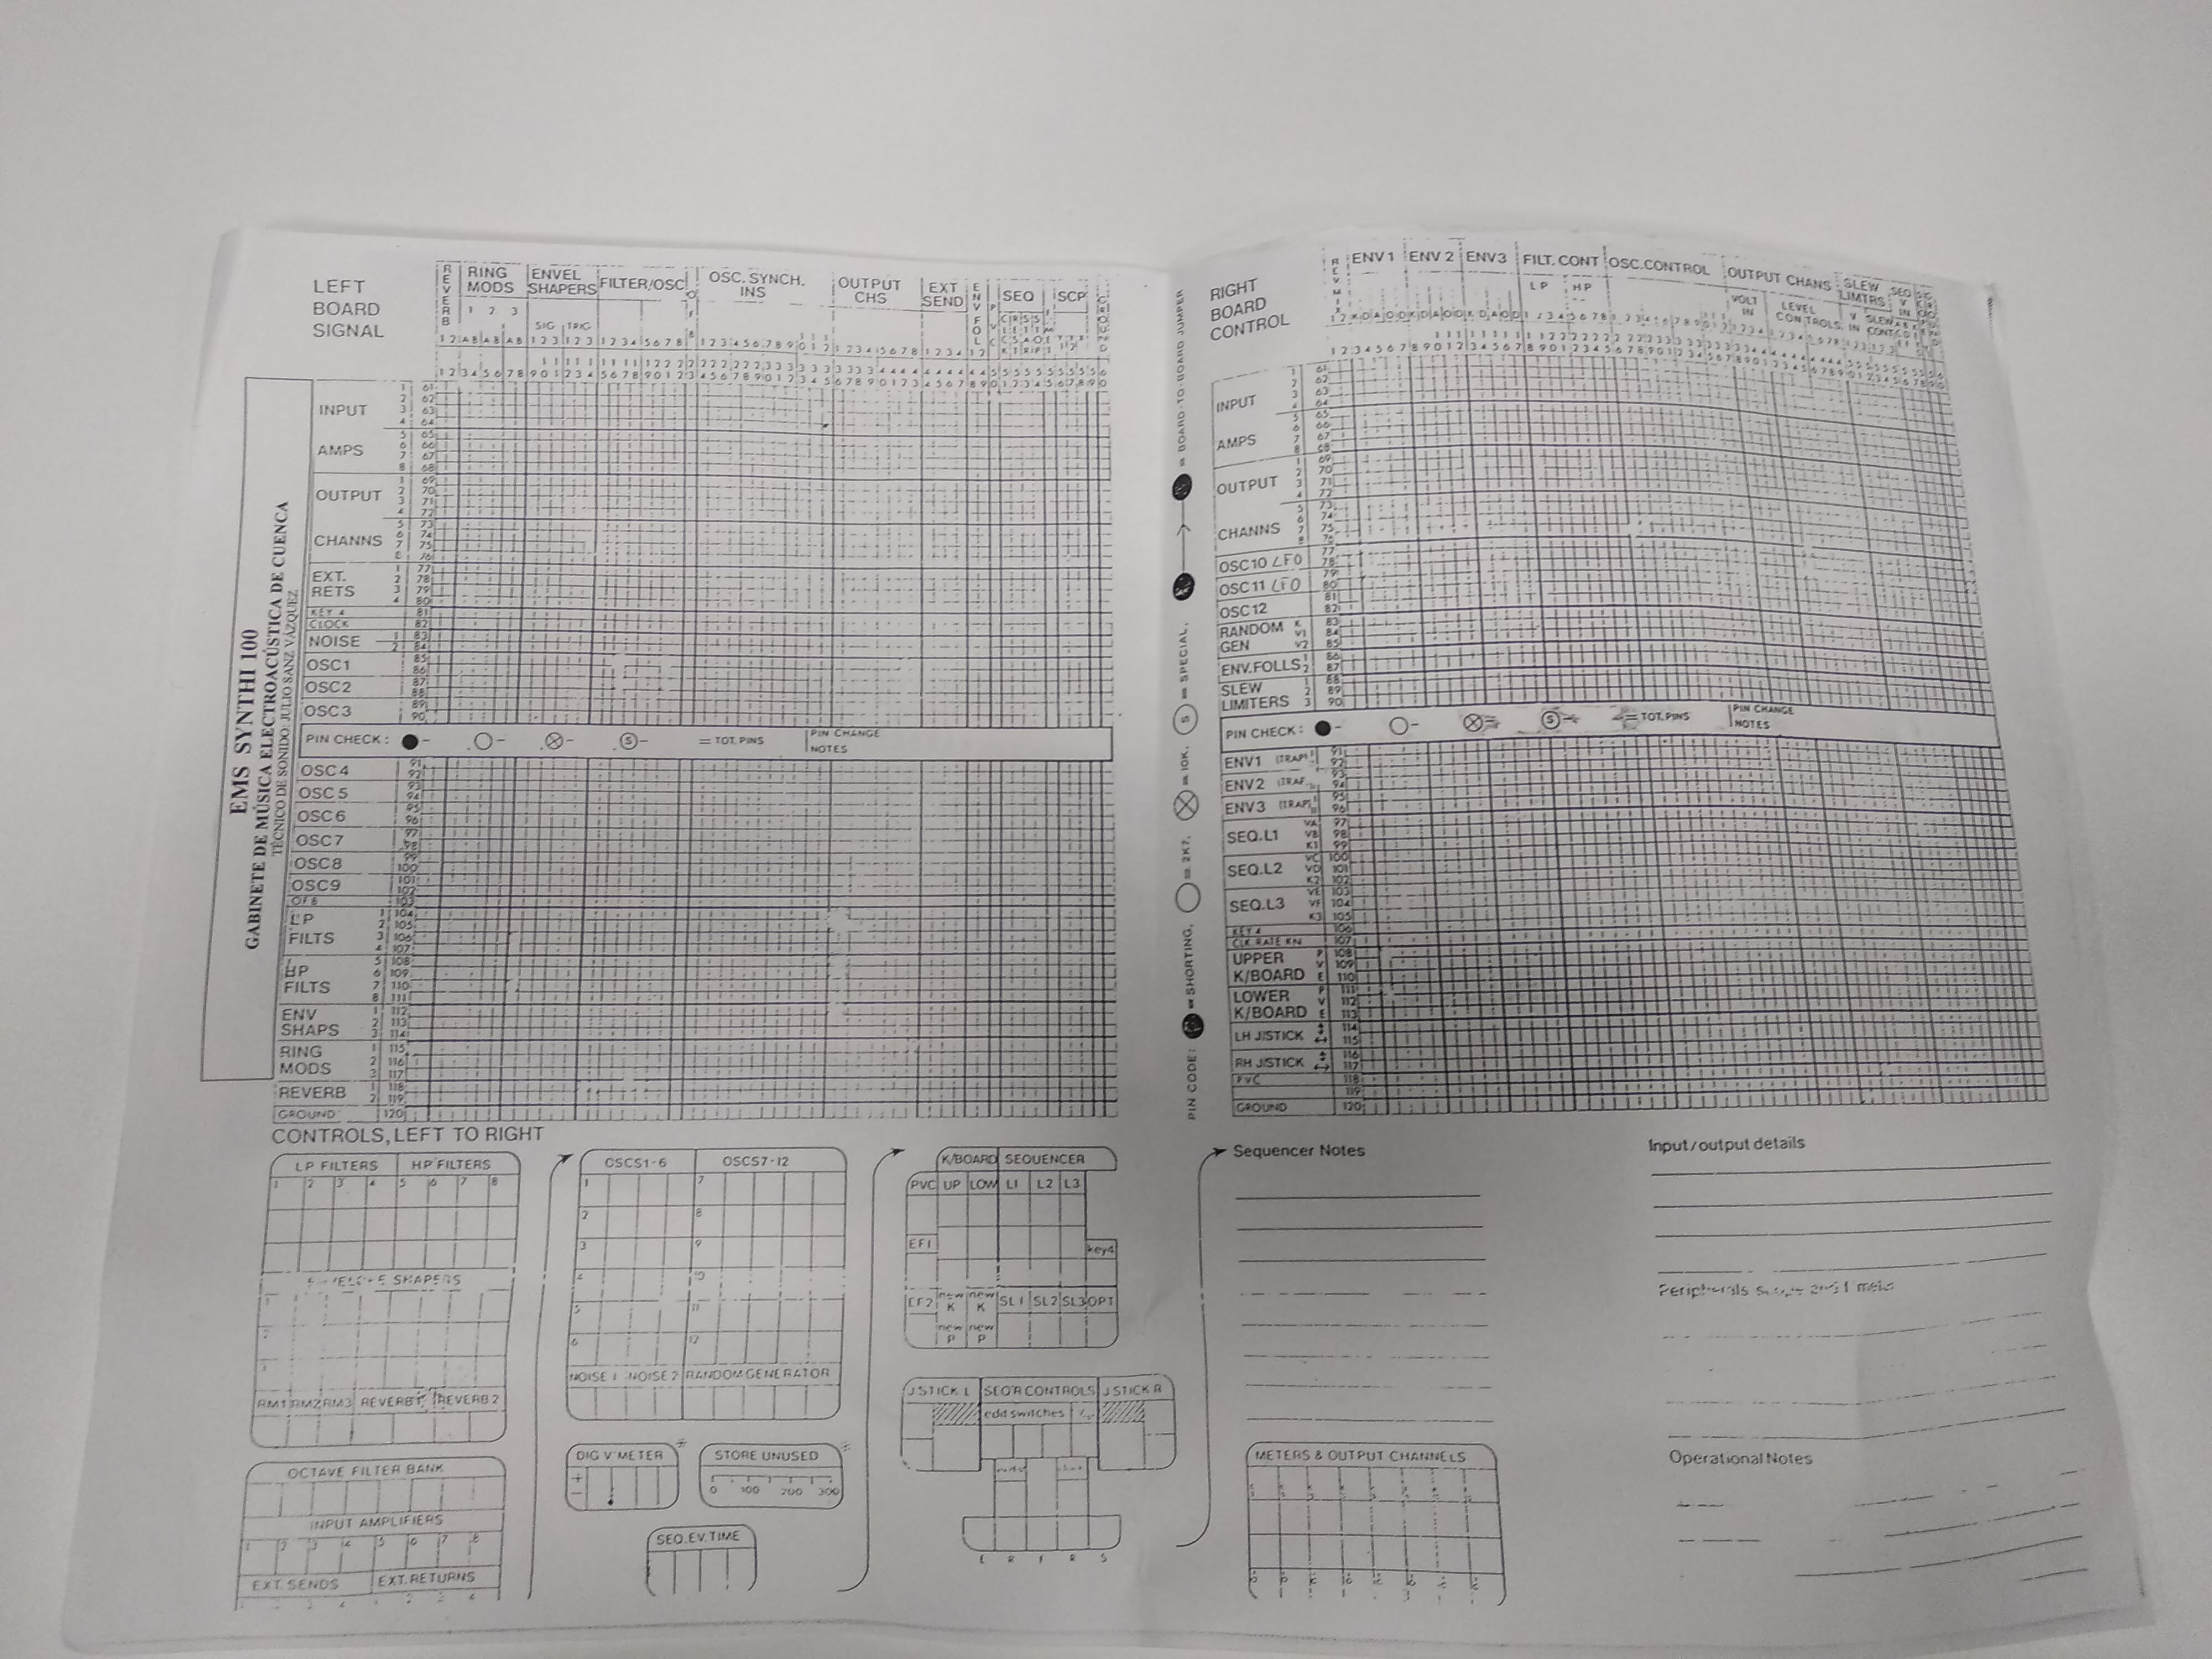
\includegraphics[width=1\textwidth]{images/dope_sheet_GME}
	\caption[\textit{Dope Sheet} conservado en el GME]{\textit{Dope Sheet} conservado en el GME, hoja en la que el compositor o el técnico encargado del GME tomaba nota esquemática de todas las conexiones y de los valores de ciertos módulos con el fin de poder repetirlos en el futuro.}
	\label{fig:dope_sheet_GME}
\end{figure}

\begin{figure}
	\centering
	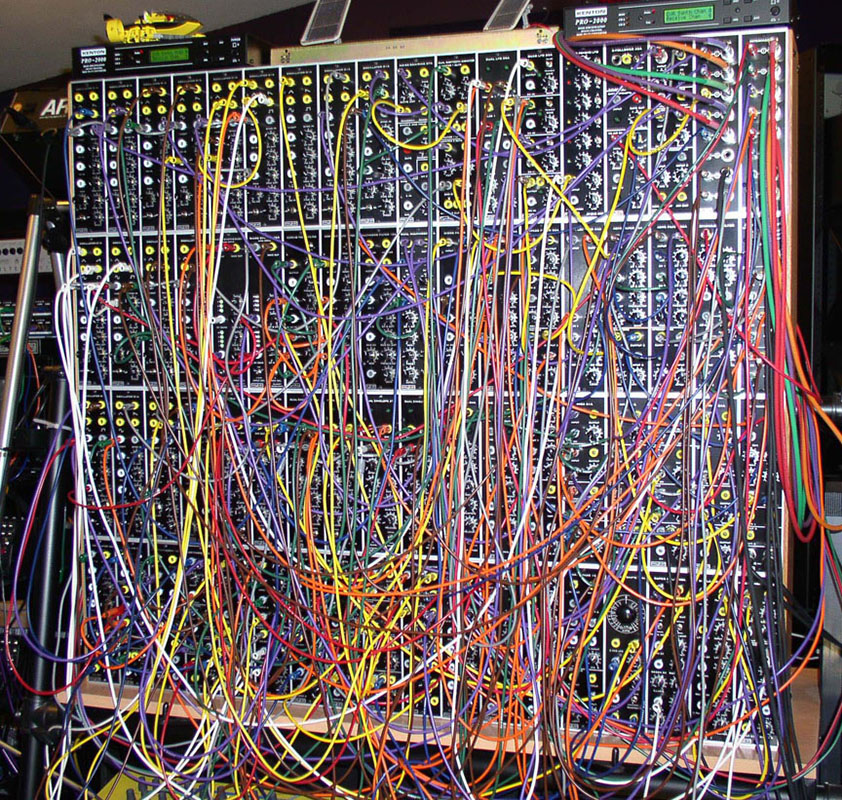
\includegraphics[width=1\textwidth]{images/sinte_modular}
	\caption[Tipico cableado de un sintetizador modular]{Tipico cableado de un sintetizador modular. Las salidas de un módulo se conectan por medio de cables con las entradas de otros módulos. La configuración del cableado determina en parte los resultados sonoros del conjunto. A pesar de lo intuitivo del sistema y su extendido uso, la complejidad de los cruces de cables le confieren una apariencia de gran complejidad.}
	\label{fig:sintetizador_modular}
\end{figure}

\begin{figure}
	\centering
	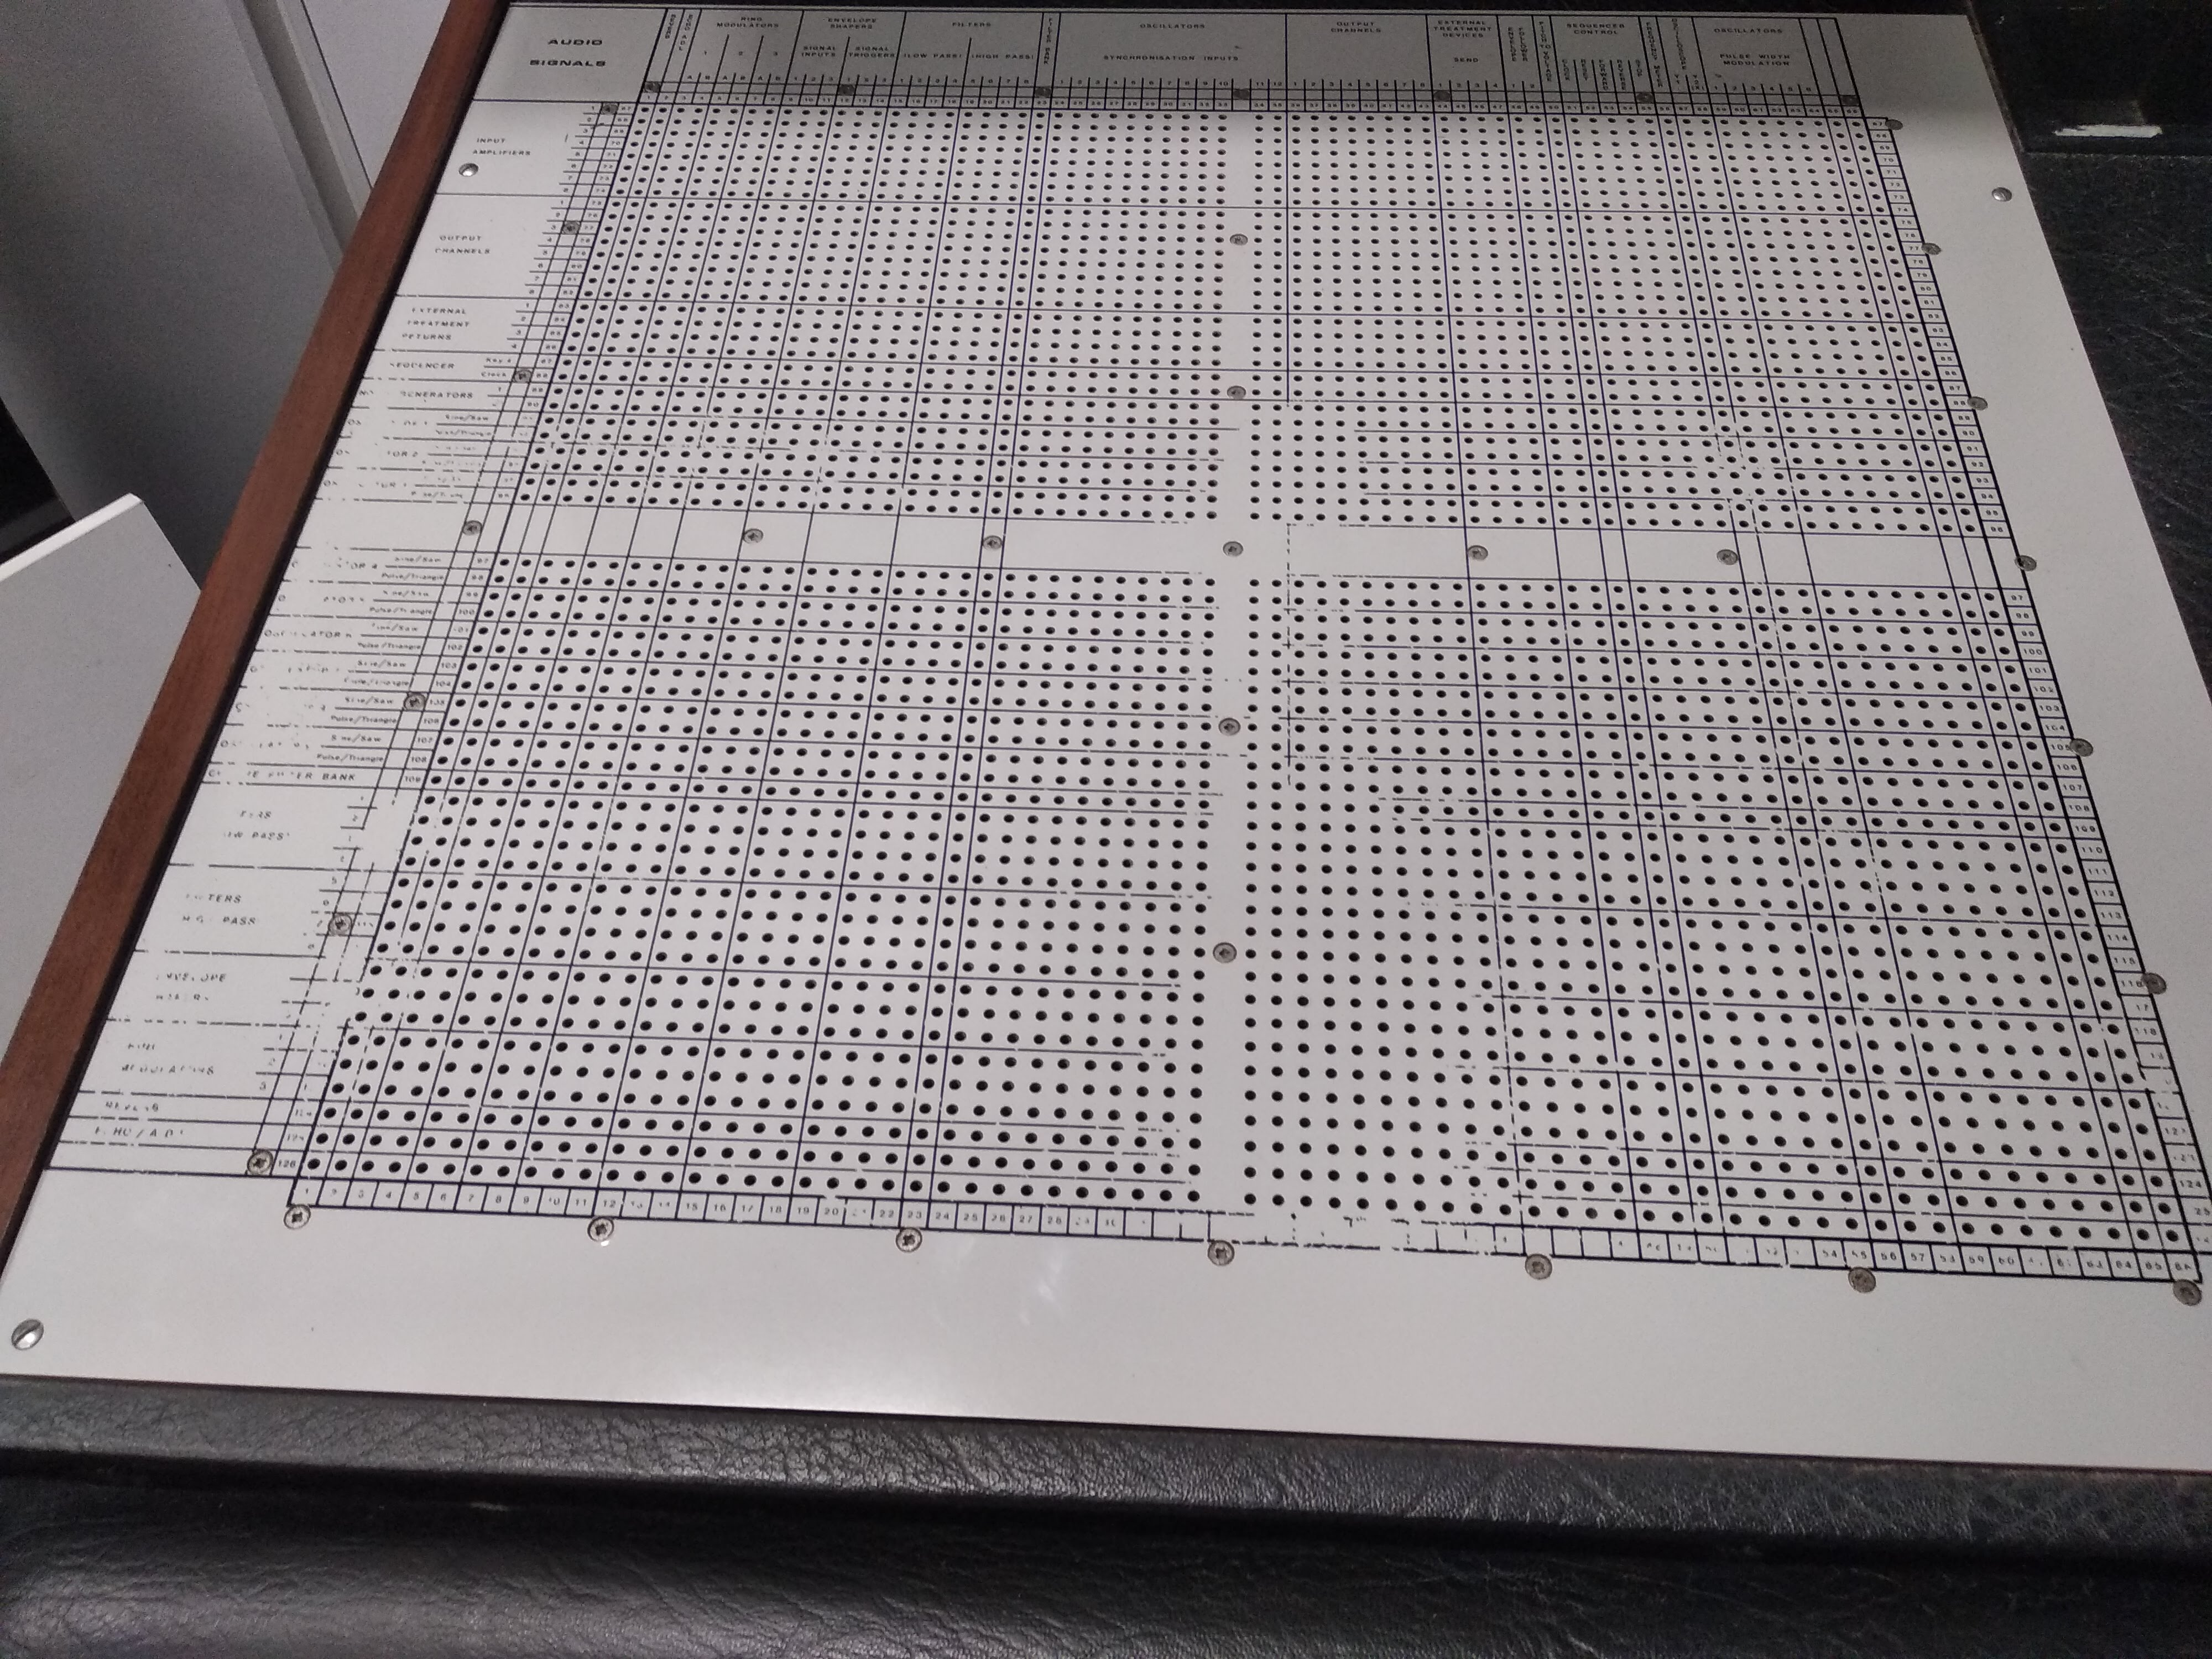
\includegraphics[width=1\textwidth]{images/patchbay_audio_vista_gral}
	\caption[Matriz \textit{Audio Control} del Synthi 100 del GME]{Matriz \textit{Audio Control} del Synthi 100 del GME. En vertical están ordenadas todas las salidas de audio de todos los módulos, mientras que en horizontal se encuentran todas las entradas. Cada nodo representa una conexión única de una entrada con una salida. Los espacios que cruzan por el centro, así como los diversos grosores de las líneas dibujadas, ayudan visualmente a situar el nodo en las coordenadas deseadas. En la fotografía se observa sensiblemente el deterioro de los textos impresos debidos al uso continuado.}
	\label{fig:patchbay_audio_vista_gral}
\end{figure}

\subsection{Implementación en \appName}

El diseño de la clase \texttt{SGME\_Patchbay} y sus herederas \texttt{SGME\_PatchbayAudio} y \texttt{SGME\_PatchbayVoltage}, ha sido uno de los que más cuidado ha requerido a la hora de crear el código. El concepto de su funcionamiento, sin embargo, es bastante simple. Cada módulo dispone de tantos \textit{busses} como entradas y salidas tenga. Al conectar un nodo de una matriz, se crea un \texttt{Synth} cuya única misión es recibir la señal de un \textit{bus} y comunicarlo a otro. De este modo, el circuito queda cerrado, y solo se abre cuando se desconecta el nodo, y con él se destruye el \texttt{Synth} que unía los \textit{busses}.

Es muy importante tener en cuenta el orden de ejecución de todos los \texttt{Synths} de la aplicación (véase \ref{sec:sc_features} para más detalles). Una conexión entre un módulo que se ejecuta más tarde que su receptor no comunicará a este ninguna señal ya que el ciclo terminará antes de que el \textit{bus} pueda conducirla a su destino, siendo eliminada antes de comenzar el siguiente ciclo. Es precisamente en las matrices donde hay que asegurar que la señal llega a su destino. Para ello se chequea la situación relativa en el servidor de los \texttt{Synths} de origen y de destino, decidiendo si se ha de leer del \textit{bus} de origen con el \textit{UGen} \texttt{In.ar} o \texttt{InFeedback.ar}


\subsubsection[Diseño de las matrices en el \textit{GUI} de  \appName]{Diseño de las matrices en el \textit{GUI} de  \appName}
Si bien se ha intentado que la apariencia gráfica de \appName~ tuviera como base fotografías del Synthi 100 de Cuenca, incluyendo sus imperfecciones en el caso de haberlas, no ha sido viable seguir este principio en el caso de las matrices, debido a que su superficie brillante y su posición horizontal hacía muy difícil la toma de fotografías sin reflejos. Además, la franja superior que contiene los textos de las entradas queda oculta en la vista cenital por los paneles verticales, ya que las matrices están ligeramente metidas bajo estos.

Se optó por dibujar ambas matrices vectorialmente (fig. \ref{fig:matriz_control_synthigme}). El dibujado de los nodos, tanto los negros como los blancos, se realiza por código desde SuperCollider. Estos han sido creados desde cero, tanto su dibujado como su comportamiento ante los clicks del ratón. En todo caso, se ha seguido escrupulosamente las proporciones de las matrices originales, así como los diversos tipos de grosores de línea, espaciados, etc.  El tipo de letra no es el mismo, si bien se ha buscado uno similar \textit{sans serif}.

\begin{figure}
	\centering
	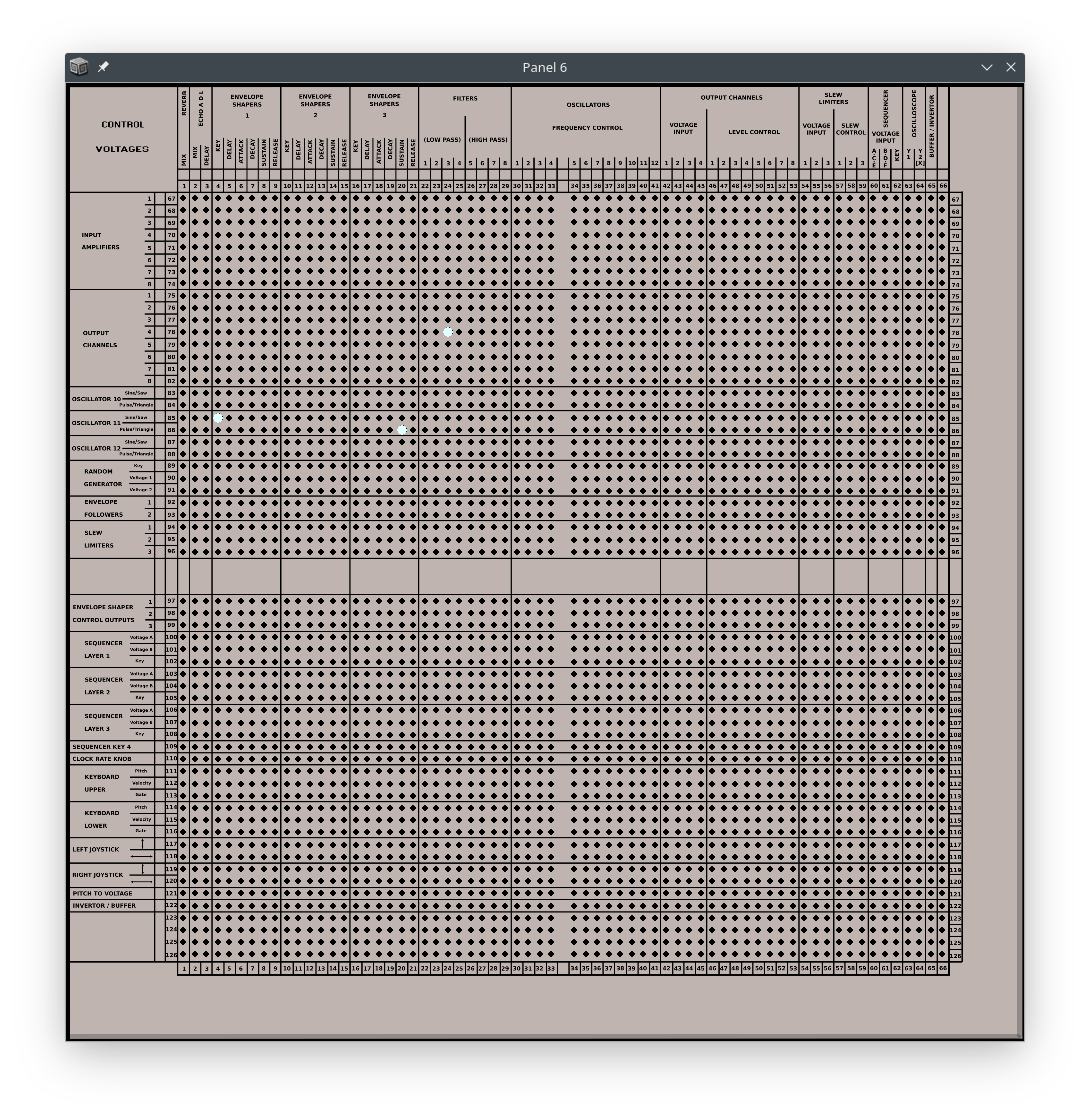
\includegraphics[width=1\textwidth]{images/matriz_control_synthigme}
	\caption[Matriz \textit{Voltage Control} de la aplicación \appName]{Matriz \textit{Voltage Control} de la aplicación \appName. Las matrices son las únicas ventanas cuya diseño no corresponde a fotografías del Synthi 100 de Cuenca, sino que son dibujos vectoriales copia del original. En la imagen se pueden apreciar tres conexiones representadas con puntos blancos.}
	\label{fig:matriz_control_synthigme}
\end{figure}

\begin{figure}
	\centering
	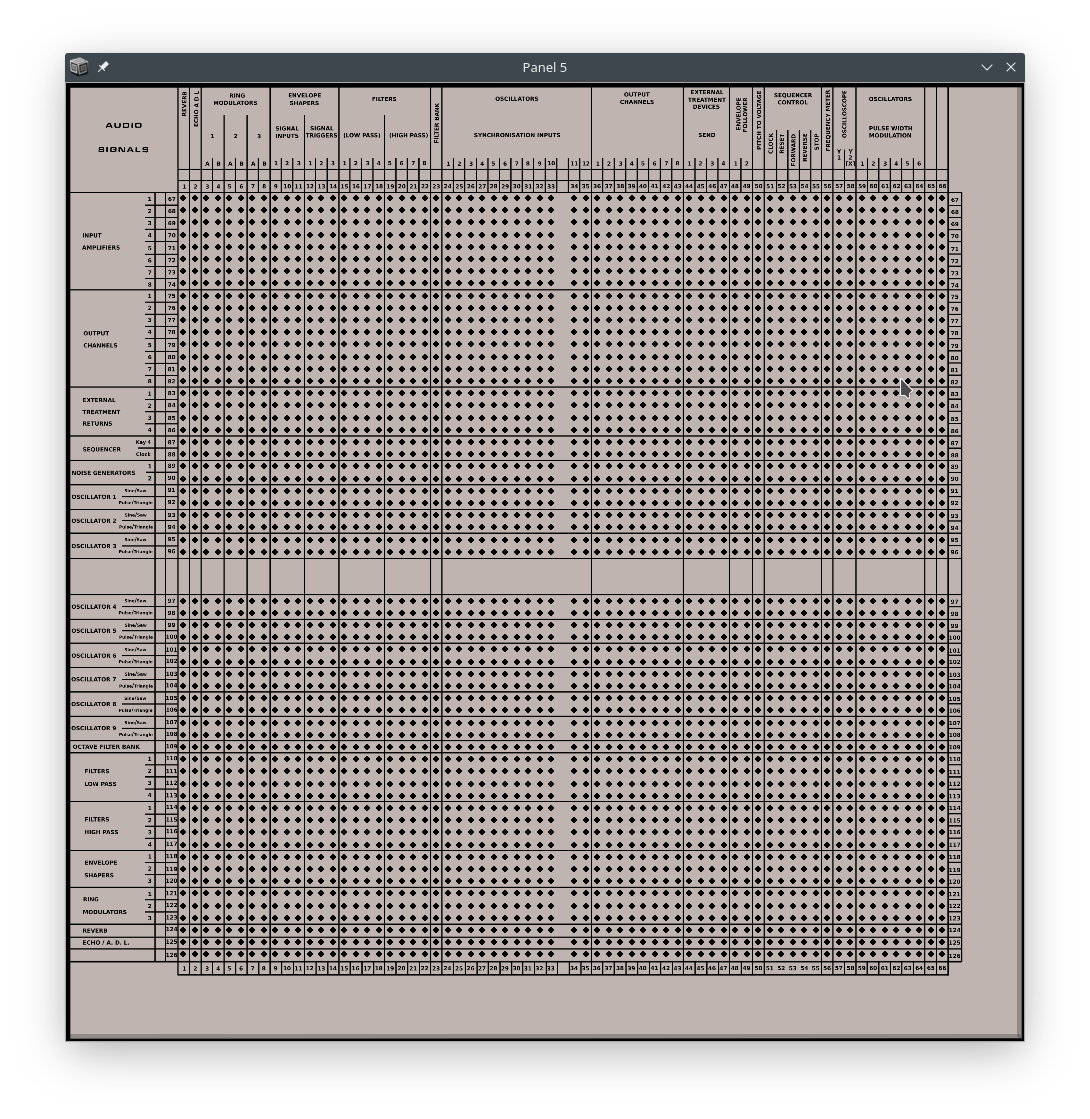
\includegraphics[width=1\textwidth]{images/matriz_audio_synthigme}
	\caption[Matriz \textit{Audio Control} de la aplicación \appName]{Matriz \textit{Audio Control} de la aplicación \appName.}
	\label{fig:matriz_audio_synthigme}
\end{figure}